\section{Auswertung}
\label{sec:Auswertung}

\begin{table}
  \centering
  \caption{Materialeigenschaften der Grundplatte. \cite{V204}}
  \label{tab:1}
  \sisetup{table-format=1.2}
  \begin{tabular}{l S S S S S }
    \toprule
    {$\text{Material}$} & {$l [\si{\centi\meter}]$} & {$b [ \si{\centi\metre}]$} & {$h[\si{\centi\metre}]$} & {$\rho [\si{\kilo\gram\per\metre\tothe{3}}$]} & {$c [\si{\joule\per\kilo\gram\per\kelvin}]$} \\
    \midrule
    Messing  & 9 & 1.2 & 0.4 & 8520 & 385 \\
    Messing  & 9 & 0.9 & 0.4 & 8520 & 385 \\
    Aluminium  & 9 & 1.2 & 0.4 & 2800 & 830 \\
    Edelstahl  & 9 & 1.2 & 0.4 & 8000 & 400 \\
    \bottomrule
  \end{tabular}
\end{table}


\subsection{statische Messung}
\label{subsec:aus_stat}
Wie in \autoref{subsec:durch_stat} beschrieben, wird eine statische Messung der Temperaturverläufe an den Stäben durchgeführt. 
Die Daten werden in folgenden Diagrammen dargestellt und ausgewertet.

\begin{figure}[H]
  \begin{subfigure}{\textwidth}
  \centering
  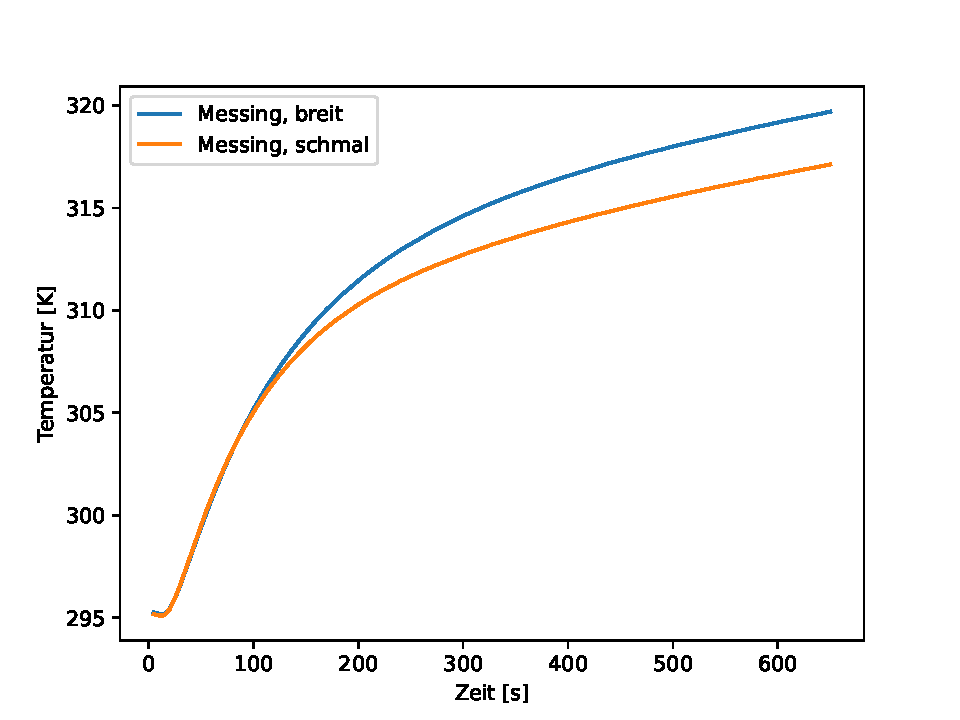
\includegraphics[height=9cm]{content/verlauf_mess.pdf}
  \caption{Temperaturverlauf der Messingstäbe (fern)}
  \label{fig:mess}
  \end{subfigure}
  \hfill
  \begin{subfigure}{\textwidth}
  \centering
  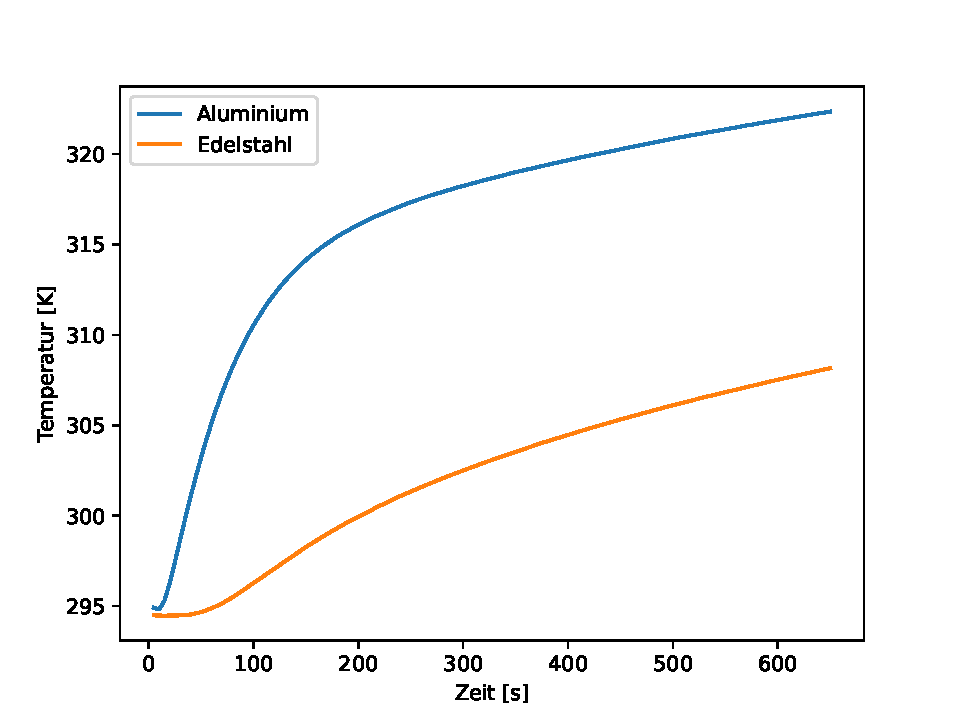
\includegraphics[height=9cm]{content/verlauf_alu_edel.pdf}
  \caption{Temperaturverlauf des Aluminium- und Edelstahlstabs (fern)}
  \label{fig:alu_edel}
  \end{subfigure}
  \caption{Temperaturverläufe der Stäbe an den fernen Thermoelementen}
  \label{fig:fern}
\end{figure}
Zunächst wurden die Temperaturen an den fernen Thermoelementen über einen Zeitraum von $\qty{650}{\second}$ aufgenommen.
Die Temperaturverläufe aller $4$ untersuchten Stäbe weisen Gemeinsamkeiten auf. So sieht man im Vergleich der Graphen in \autoref{fig:fern},
dass bei allen Metallen die Temperatur initial stark steigt und sich mit zunehmender Zeit einem Sättigungswert annähert.
Der Temperaturanstieg ist bei Edelstahl allerdings deutlich langsamer als bei den übrigen Metallen und auch der Sättigungswert ist hier deutlich niedriger.
Bei den beiden Messingstäben sind sehr ähnliche Temperaturverläufe zu beobachten, wobei die Kurve des breiten Stabs zu einem späteren Zeitpunkt abflacht als die des schmalen Stabs.


\begin{table}[H]
  \centering
  \caption{Temperaturen der Stäbe nach 650s}
  \label{tab:650s}
  \begin{tabular}{l S[table-format=3.2]}
    \toprule
    {Material} & {Temperatur [K]}\\
    \midrule
    {Messing, breit} & 319.70\\
    {Messing, schmal} & 317.12\\
    {Aluminium} & 322.35\\
    {Edelstahl} & 308.15\\
    \bottomrule
  \end{tabular}
\end{table}
Zur Bewertung der Wärmeleitung der Stäbe wurde die Temperatur am Ende der statischen Messung erhoben und in einer Tabelle dargestellt.
Aus den Werten in \autoref{tab:650s} lässt sich erkennen, dass Aluminium von den untersuchten Metallen die beste Wärmeleitfähigkeit besitzt
und Edelstahl die Wärme am schlechtesten leitet.

\begin{table}[H]
  \centering
  \caption{Wärmeströme zu verschiedenen Messzeiten}
  \label{tab:dQ/dt}
  \sisetup{table-format=3.3}
  \begin{tabular}{S[table-format=3.0] S S S S}
    \toprule
    & \multicolumn {4}{c}{Wärmestrom $\Delta Q \mathbin{/}\Delta t \, [\si{\watt}]$}\\
    \cmidrule(lr){2-5}
    \multicolumn{1}{c}{Messzeitpunkt $t$ [$\si{s}$]}& \multicolumn{1}{c}{Messing, breit} & \multicolumn{1}{c}{Messing, schmal}  & \multicolumn{1}{c}{Aluminium} & \multicolumn{1}{c}{Edelstahl}\\
    \midrule
    50 &-1.235&-0.879&-2.067&-0.268\\
    200 &-0.669&-0.520&-0.846&-0.395\\
    350 &-0.476&-0.425&-0.645&-0.354\\
    500 &-0.427&-0.404&-0.599&-0.332\\
    650 &-0.409&-0.398&-0.592&-0.320\\
    \bottomrule
  \end{tabular}
\end{table}
In der \autoref{tab:dQ/dt} sind die mithilfe von \autoref{eqn:Wärmemenge} berechneten Wärmeströme der
verschiedenen Metalle zu fünf unterschiedlichen Messzeitpunkten zu sehen.

\begin{figure}[!htbp]
  \begin{subfigure}{\textwidth}
  \centering
  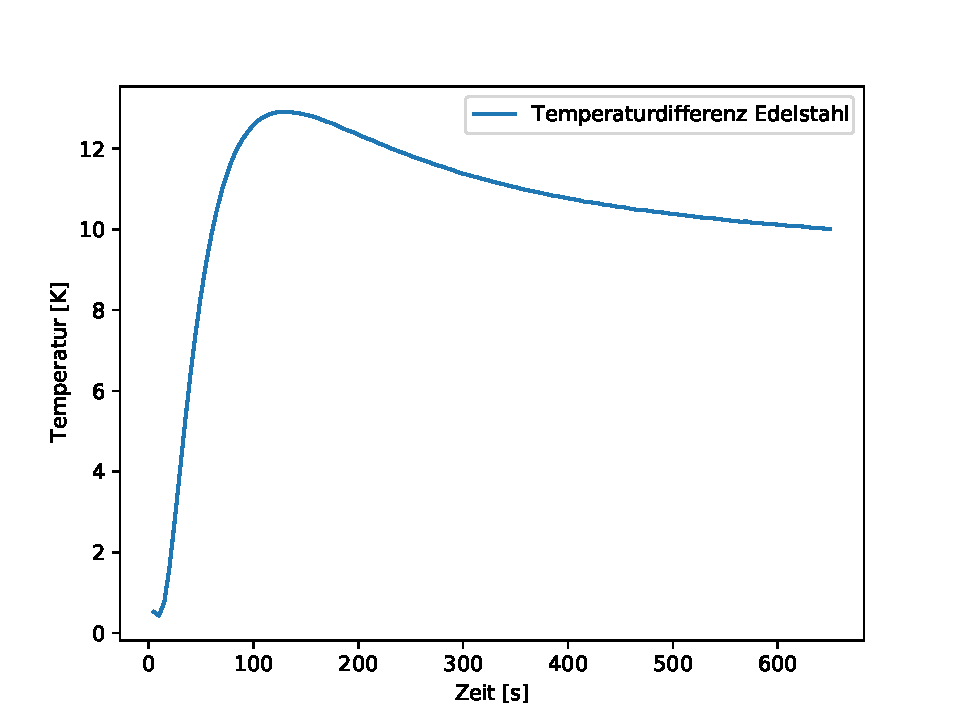
\includegraphics{content/differenz_edel.pdf}
  \caption{Verlauf der Temperaturdifferenz am Edelstahlstab}
  \label{fig:diff_edel}
\end{subfigure}
\begin{subfigure}{\textwidth}
  \centering
  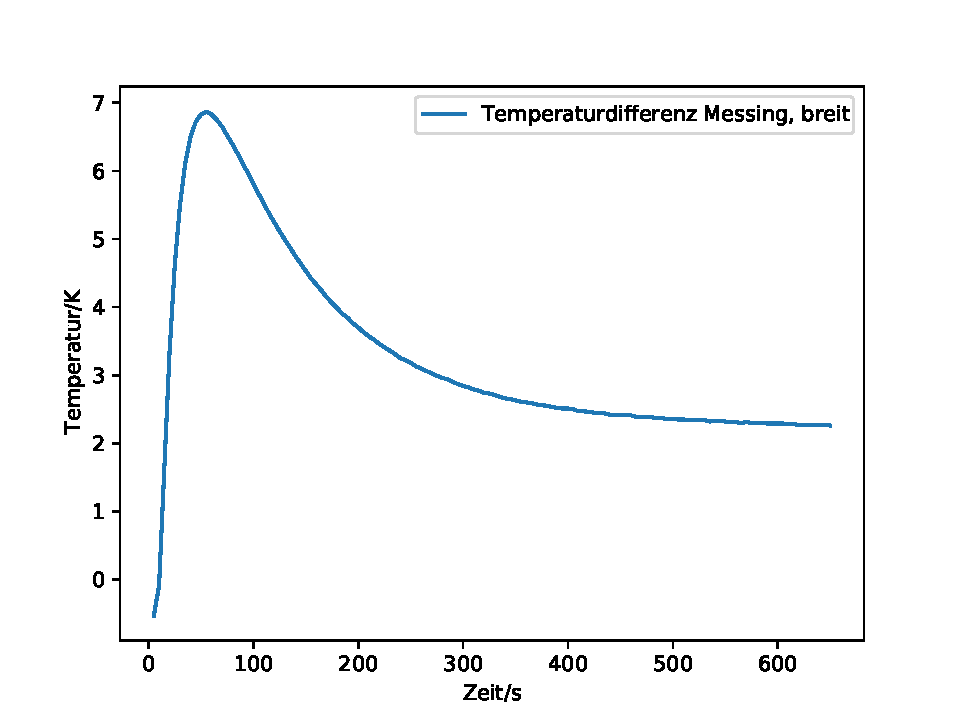
\includegraphics{content/differenz_mess.pdf}
  \caption{Verlauf der Temperaturdifferenz am breiten Messingstab}
  \label{fig:diff_mess}
\end{subfigure}
\caption{Verlauf der Temperaturdifferenzen zwischen den Thermoelementen}
\label{fig:diff}
\end{figure}

In \autoref{fig:diff} sind die Verläufe der Temperaturdifferenzen zwischen den Thermoelementen auf dem breiten Messingstab, sowie dem Edelstahlstab dargestellt.
Es lässt sich erkennen, dass die Differenz bei beiden Stäben zunächst stark ansteigt , dann aber einen Hochpunkt aufweist und danach wieder fällt,
sich dann aber einem Sättigungswer annähert und die Kurven abflachen. 
Beim Messingstab ist die Differenz allerdings ab dem Hochpunkt der Kurve deutlich niedriger als beim Edelstahlstab.
Auch beträgt die Temperaturdifferenz am Hochpunkt der Kurve bei Edelstahl einen Wert von über 12 K, wobei der Wert am Hochpunkt der Messingkurve unter 7 K liegt.

\subsection{Dynamische Messung}
\label{aus_dyn}

Wie in \autoref{subsec:durch_dyn} beschrieben, werden mehrere dynamische Messungen der Temperaturverläufe an den Stäben durchgeführt. 
Die Daten werden in folgenden Diagrammen dargestellt und ausgewertet.

Zunächst wurde die Messung nach dem Angström-Verfahren, siehe \autoref{sec:Durchführung} mit einer Periodendauer von $\qty{80}{\second}$ durchgeführt.
Die Werte an den Thermoelementen am breiten Messingstab und am Aluminiumstab werden in \autoref{fig:mess_dyn} und \autoref{fig:alu_dyn} dargestellt.
Anhand der Graphen wurden die Amplituden, sowie die Phasendifferenzen aus den Abständen der Wellenhochpunkte beider Wellen bestimmt.
Außerdem wurde nach \autoref{eqn:kappa} die Wärmeleitfähigkeit $\kappa$ der verschiedenen Metalle berechnet. Die Ergebnisse sind in \autoref{tab:kappa} aufgelistet.
\begin{figure}[!htbp]
  \centering
  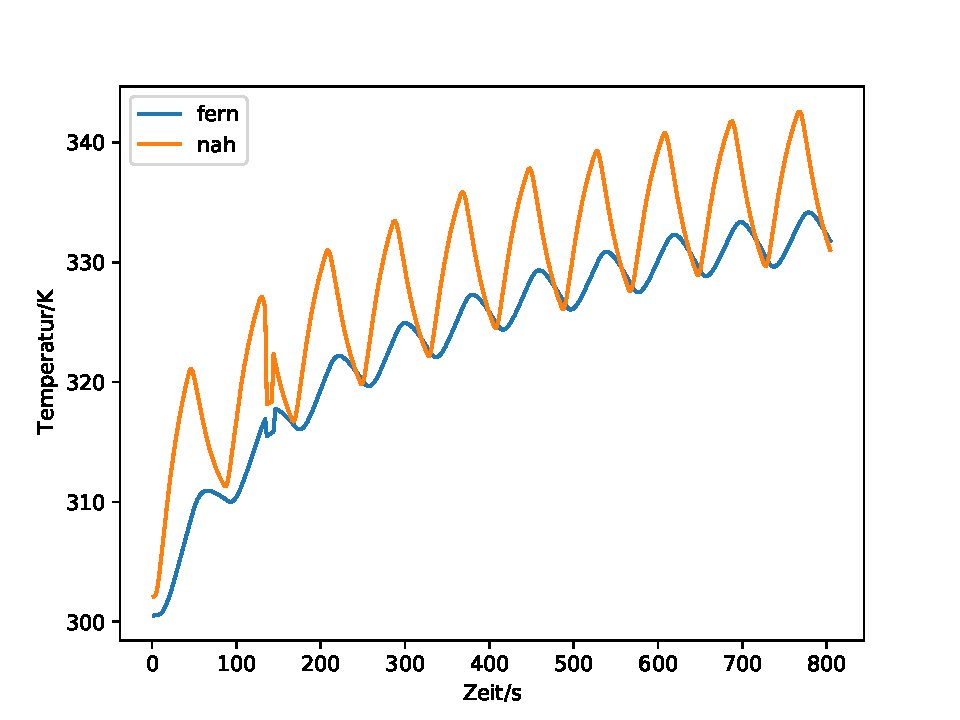
\includegraphics{content/dyn_80_mess.pdf}
  \caption{Temperaturverlauf des breiten Messingstabs}
  \label{fig:mess_dyn}
\end{figure}
\begin{figure}[!htbp]
  \centering
  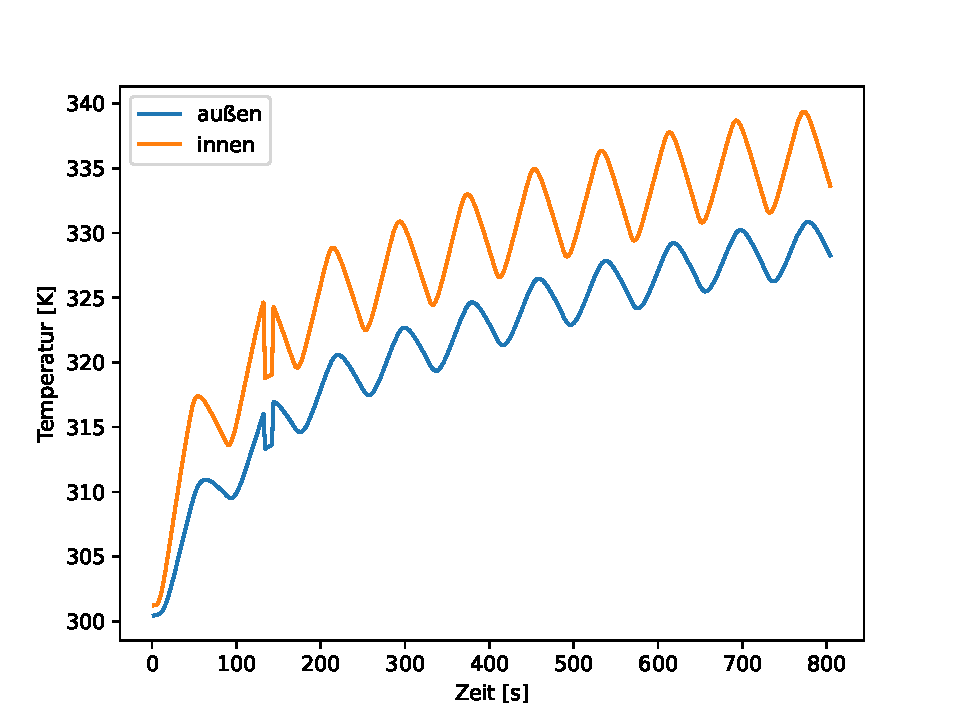
\includegraphics{content/dyn_80_alu.pdf}
  \caption{Temperaturverlauf des Aluminiumstabs}
  \label{fig:alu_dyn}
\end{figure}
	
\begin{table}[H]
	\centering
	\caption{Amplituden und Phasendifferenzen Messing und Aluminium}
	\label{tab:AuP}
  \sisetup{table-format=2.3}
	\begin{tabular}{l S S S[table-format=2.0] S S S[table-format=2.0]}
		\toprule
    & \multicolumn{3}{c} {Messing} & \multicolumn{3}{c} {Aluminium}\\
    \cmidrule(lr){2-4}\cmidrule(lr){5-7}
		&{$A_{nah}$ [K]} & {$A_{fern}$ [K]} &{$\Delta t [\si{\second}]$}&{$A_{nah}$ [K]} & {$A_{fern}$ [K]} &{$\Delta t [\si{\second}]$}\\
		\cmidrule(lr) {2-4}\cmidrule(lr) {5-7}
		&9.5&5.21&20   & 11.51 & 8.075 & 10 \\
    &7.91&3.865&16 & 9.43 & 5.505 & 4 \\
    &7.16&3.07&14  &8.46 & 4.64 & 6 \\
    &6.83&2.635&12 & 8.19 & 4.18 & 8 \\
    &6.865&2.61&12 & 8.12 & 4.28 & 8 \\
    &6.67&2.48&10  & 8.05 & 4.19 & 8 \\
    &6.595&2.41&10 & 7.965 & 4.095 & 6 \\
    &6.615&2.395&10& 7.98 & 4.19 & 8 \\
    &6.405&2.225&10& 7.805 & 3.95 & 6 \\
    &6.45&2.265&10 & 7.817 & 3.915 & 6 \\
    \cmidrule(lr) {2-4}\cmidrule(lr) {5-7}
    {Mittelwert}&7.1 &2.920 &12.4 & 8.533 & 4.702 & 7.0\\
		\bottomrule
	\end{tabular}
\end{table}	

Aus den Werten in \autoref{tab:AuP} kann mithilfe von \autoref{eqn:kappa} die Wärmeleitfähigkeit berechnet werden.
Der Fehler wird nach der Gauß'schen Fehlerfortpflanzung mit: 
\begin{equation}
  \label{eqn:Gauß}
  \Delta \kappa = \sqrt{\biggl(\frac{\partial \kappa}{\partial \Delta t}\biggr)^2\cdot (\Delta (\Delta t))^2+
  \biggl(\frac{\partial \kappa}{\partial A_\text{nah}}\biggr)^2\cdot (\Delta  A_\text{nah} )^2+
  \biggl(\frac{\partial \kappa}{\partial A_\text{fern}}\biggr)^2\cdot (\Delta  A_\text{fern})^2} 
 \end{equation}

Diese beträgt:
\begin{align*}
  \kappa_{\text{Messing}}&=\qty{133.95 +- 63.92}{\watt\per\meter\per\kelvin}\\
  \kappa_{\text{Aluminium}}&=\qty{250.72 +- 140.93}{\watt\per\meter\per\kelvin}
\end{align*}

\begin{figure}[!htbp]
  \centering
  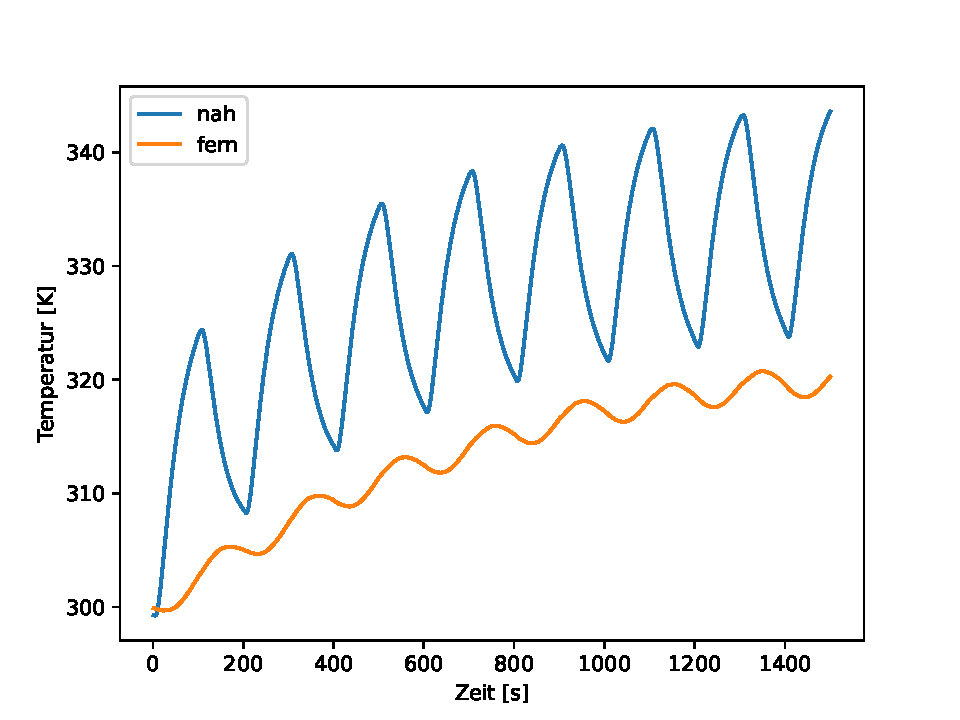
\includegraphics{content/dyn_2.pdf}
  \caption{Temperaturverlauf des Edelstahlstabs}
  \label{fig:edel_dyn}
\end{figure}

\begin{table}[H]
	\centering
	\caption{Amplituden und Phasendifferenzen Edelstahl}
	\label{tab:AuPE}
  \sisetup{table-format=2.3}
	\begin{tabular}{l S S S[table-format=2.0]}
		\toprule
		&{$A_{nah}$ [K]} & {$A_{fern}$ [K]} &{$\Delta t [\si{\second}]$}\\
		\cmidrule(lr) {2-4}
		& 12.57 & 2.81& 64 \\
    & 11.39& 2.56 & 64\\
    &10.85& 2.17 & 54\\
    & 10.585 & 2.065 & 50 \\
    & 10.365& 1.885& 50\\
    & 10.205& 1.665& 46\\
    & 10.158& 1.595 & 40\\
    \cmidrule(lr) {2-4}
    {Mittelwert}&10.879&2.107 &52.571 \\
		\bottomrule
	\end{tabular}
\end{table}	

Auch zur Berechnung der Wärmeleitfähigkeit von Messing und Aluminium wird nun auch die Wärmeleitfähigkeit von Edelstahl berechnet.
\begin{align*}
  \kappa_{\text{Edelstahl}}&=\qty{10.97 +- 1.52}{\watt\per\meter\per\kelvin}\\
  \end{align*}

Wellenlänge, Frequenz
Nach \autoref{eqn:welle} lassen sich die Wellenlängen der Temperaturwellen bestimmen. Wobei $T=\frac{1}{f}$ die Periodendauer und $f$ die Frequenz der Welle beschreibt.
\begin{equation*}
  \label{eqn:welle}
  \lambda = \sqrt{\frac{4 \pi \kappa T}{\rho c}}
\end{equation*}





